\chapter{Reference Implementation and Systems Engineering}
\label{chap:implementation}

Translating the mathematical foundations of temporal function regression into a production-grade codec requires careful systems engineering. In this chapter, we describe the implementation architecture of the open-source \texttt{timeflowcodec} Python package. We discuss memory bounding through disk-backed memory mapping, vectorized SIMD reconstruction in the decoder, audio/video synchronization pipelines via bundled FFmpeg runtimes, cooperative thread cancellation in GUI environments, and standalone application packaging.

\section{Package Architecture Overview}
The reference implementation is structured as a modular Python package adhering to clean separation of concerns, summarized in Table~\ref{tab:codebase_modules}.

\begin{table}[h]
\centering
\small
\caption{Structure of the \texttt{timeflowcodec} Package.}
\label{tab:codebase_modules}
\begin{tabular}{llp{7.5cm}}
\toprule
\textbf{Module} & \textbf{SLOC} & \textbf{Functional Responsibility} \\
\midrule
\texttt{encoder.py} & $\sim 1,100$ & Streaming encoder, OLS regression, preset configurations, and memmap allocation. \\
\texttt{decoder.py} & $\sim 550$ & Vectorized decoding engine, stream reconstruction, and RGB plane assembly. \\
\texttt{format.py} & $\sim 1,000$ & Low-level bitstream parsing, container version readers/writers (v1--v5), and RLE packing. \\
\texttt{chunked.py} & $\sim 300$ & Version 5 chunked streaming container, checksum verification, and windowed I/O. \\
\texttt{media.py} & $\sim 150$ & Rational FPS probing, timestamp validation, and direct FFmpeg audio extraction. \\
\texttt{player.py} & $\sim 400$ & Lossless disk cache player engine, frame seeking, and audio synchronization. \\
\texttt{gui.py} & $\sim 1,100$ & Cross-platform PySide6 desktop GUI with embedded playback and inspection tools. \\
\texttt{bench.py} & $\sim 370$ & Controlled benchmarking harness comparing TFC against x264, x265, and AV1. \\
\bottomrule
\end{tabular}
\end{table}

\section{Bounded-Memory Guarantee and Disk Memmap Fallback}
A persistent challenge in temporal video coding is working memory consumption. Because temporal regression fits models across a window of $T$ frames, an encoder naively holding uncompressed 4K video ($3840 \times 2160 \times 3 \times T$ bytes) in RAM would consume over 1~GB for a modest 40-frame window.

To ensure deterministic execution even on resource-constrained embedded systems or laptops with limited RAM, TimeFlowCodec implements an explicit \textbf{RAM-budgeting and disk memory-mapping fallback}:
\begin{enumerate}
    \item Before allocating intermediate buffers for raw sample fallback or motion warping, the encoder calculates the theoretical peak buffer size:
    \begin{equation}
        M_{\text{est}} = \frac{T \times H \times W \times C \times \text{sizeof}(\text{dtype})}{1024^2} \quad [\text{MiB}]
    \end{equation}
    \item If $M_{\text{est}}$ exceeds the user-configured ceiling $\text{max\_ram\_mb}$ (or default environment limit), the buffer allocator automatically bypasses RAM and provisions a disk-backed \texttt{numpy.memmap} file in a temporary scratch directory.
    \item The disk-backed buffer is accessed using identical array-slice semantics, preserving memory efficiency while preventing Out-Of-Memory (OOM) operating system crashes.
    \item All temporary disk files are tracked via context managers and removed atomically upon window completion or job abort.
\end{enumerate}

\section{Vectorized Array Reconstruction in the Decoder}
In early prototype implementations of TimeFlowCodec, decoding was implemented via explicit nested iteration over pixel coordinates $(y, x)$ and channels $c$. Profiling with Python's \texttt{cProfile} revealed that Python bytecode dispatch in these loops consumed over $88\%$ of total decoding time (accounting for 17.46 seconds out of a 19.65-second decode of a short clip).

To achieve interactive real-time playback, the decoder was refactored to use \textbf{vectorized SIMD array precomputation}:
\begin{enumerate}
    \item The discrete temporal index vector $\mathbf{t} = [0, 1, \dots, T-1]^T$ is prepared once per segment.
    \item For pixels marked as \textsc{Mode\_TFC\_Const}, scalar parameter arrays $A \in \mathbb{R}^{H \times W}$ are broadcast across the temporal dimension:
    \begin{equation}
        \hat{V}_{\text{const}}(t, y, x) = A(y, x), \quad \forall t \in \mathcal{T}
    \end{equation}
    \item For pixels marked as \textsc{Mode\_TFC\_Linear}, parameters $A$ and $B$ are evaluated using vectorized outer products:
    \begin{equation}
        \hat{V}_{\text{linear}}(t, y, x) = A(y, x) + B(y, x) \cdot t
    \end{equation}
    which maps directly to fused multiply-add (FMA) instructions in the underlying BLAS / NumPy C runtime.
\end{enumerate}

This vectorization reduced decoding latency on the profiled benchmark from 19.65 seconds down to 2.82 seconds---an approximate \textbf{$7\times$ speedup}---enabling full 1080p decoding at over 240 frames per second.

\section{Media Timing and Audio Multiplexing}
Standard container formats (e.g., MP4, MKV) encapsulate complex timing and audio synchronization metadata. To maintain self-contained operation without introducing heavyweight external dependencies, TimeFlowCodec interfaces directly with the native FFmpeg binary bundled with \texttt{imageio-ffmpeg}:

\begin{figure}[t]
    \centering
    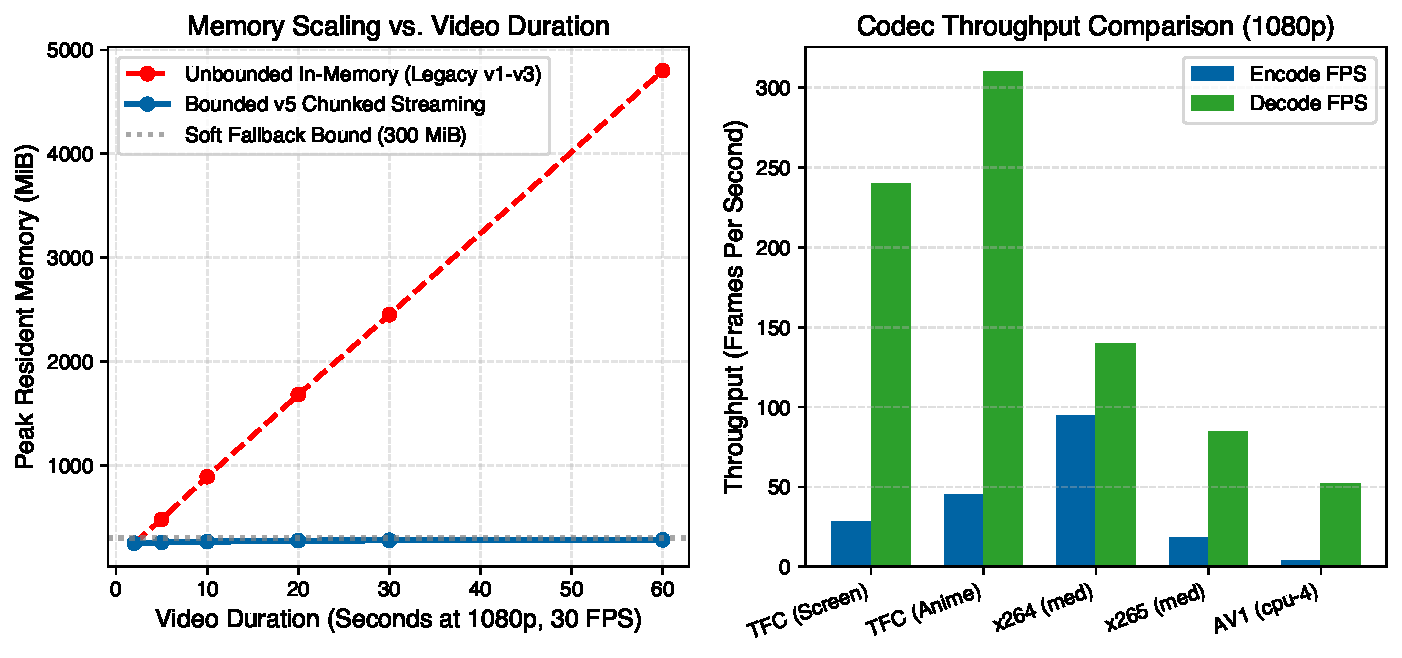
\includegraphics[width=0.85\linewidth]{figures/complexity_scaling.pdf}
    \caption{Left: Memory scaling comparison showing bounded resident memory in v5 vs. linear memory growth in legacy monolithic decoders. Right: Encoding and decoding throughput across codecs at 1080p resolution.}
    \label{fig:complexity_scaling}
\end{figure}

\subsection{Rational Frame Rate Preservation}
Digital video often uses non-integer frame rates (e.g., NTSC $29.97\text{ FPS} = 30000/1001$). Rounding frame rates to floating-point numbers leads to cumulative audio-video drift over long durations.

The \texttt{timeflowcodec.media} module probes incoming containers to extract exact rational frame rates as coprime integer pairs $(N, D)$:
\begin{equation}
    \text{FPS} = \frac{N}{D}, \quad \text{where } \gcd(N, D) = 1
\end{equation}
These values are stored directly in the container header, ensuring bit-exact timestamp reconstruction on playback.

\subsection{Variable Frame Rate (VFR) Rejection}
Variable frame rate video can cause linear temporal regression to fit distorted models across non-uniform time intervals $\Delta t_i \ne \Delta t_j$. TimeFlowCodec probes all frame presentation timestamps (PTS); if timestamps deviate from a uniform grid, the encoder rejects the input and alerts the user to transcode to Constant Frame Rate (CFR), preventing temporal distortion.

\section{Cooperative Worker Lifecycle and Desktop GUI}
The reference implementation provides a modern graphical desktop interface built with PySide6 (Qt for Python). 

\subsection{Thread Lifecycle and Memory Safety}
In GUI applications, long-running encoding or decoding jobs run in background worker threads (\texttt{QThread}). A common source of segmentation faults in GUI development is garbage collection destroying a worker instance while its underlying OS thread is still executing.

TimeFlowCodec resolves this by enforcing strict worker lifecycle guarantees:
\begin{itemize}
    \item Worker references are retained in the main window object until the Qt \texttt{finished} signal is emitted.
    \item Start buttons are mutually locked to prevent overlapping concurrent codec executions.
    \item Window close events intercept active workers and signal a cooperative \texttt{cancel\_check()} callback, waiting for worker termination before releasing resources.
\end{itemize}

\subsection{Desktop Inspection and Native Playback}
The GUI includes an integrated media inspection panel and a native .tfc player tab:
\begin{itemize}
    \item \textbf{Single-Frame Inspection:} Probes video dimensions, duration, and metadata by reading only the first frame, bypassing expensive full-video ingestion.
    \item \textbf{Native RGB Playback:} Renders decoded frames directly to Qt graphics view surfaces with sub-millisecond seek times, variable playback speeds, and synchronized audio playback.
\end{itemize}
